\documentclass{article}

\usepackage[utf8]{inputenc}

\usepackage{nicefrac}
\usepackage{amssymb, amsmath, amsfonts}
\usepackage{amsthm}
\usepackage{tikz}
\usetikzlibrary{matrix,shapes,arrows, calc, intersections}
\usetikzlibrary{decorations.markings}
\usepackage{pgfplots}
\usepackage{tkz-euclide}
\usetkzobj{angles} % important you want to use angles
\usepgfplotslibrary{groupplots}
\usepackage[a4paper, margin=1in]{geometry}

\newtheorem{proposition}{Proposition}
\newtheorem{theorem}{Theorem}
\newtheorem{definition}{Definition}
\newtheorem{lemma}{Lemma}
\newtheorem{conjecture}{Conjecture}
\newtheorem{corollary}{Corollary}
\newtheorem{remark}{Remark}
\newtheorem{assumption}{Assumption}

\newlength\figureheight
\newlength\figurewidth
\setlength\figureheight{12cm}
\setlength\figurewidth{14cm}

\newcommand{\tikzdir}[1]{tikz/#1.tikz}
\newcommand{\inputtikz}[1]{\input{\tikzdir{#1}}}

\DeclareMathOperator*{\argmin}{arg\; min}     % argmin
\DeclareMathOperator*{\argmax}{arg\; max}     % argmax
\DeclareMathOperator*{\tr}{tr}     % trace
\DeclareMathOperator{\Cov}{Cov}
\DeclareMathOperator{\logdet}{log\;det}

\title{EE8087 Living with Mathematics\\Tutorial 5: Astronomy}
\date{}
\begin{document} \maketitle
\begin{enumerate}
\item Suppose Earth is a perfect sphere with radius $6371$km. A sailor is standing on the top of a mast $10$m above sea level. Can she see a light tower $30$km away and $20$m above sea level?

\begin{figure}[ht]
  \centering
  \begin{tikzpicture}
    \tkzDefPoint[label=135:$A$](-0.6,3){A}
    \tkzDefPoint[label=180:$O$](0,0){O}
    \tkzDefPoint[label=45:$B$](1,3){B}
    \tkzDefPoint[label=90:$P$](0,3){P}
    \tkzDrawCircle[R](O,3 cm)
    \tkzDrawSegments(O,A O,B O,P A,B)
    \tkzDrawPoints(A,B,O,P)
  \end{tikzpicture}
\end{figure}

\emph{Soln:} Suppose the sailor is standing at point $A$. We know that $OA = R + h_1$, where $R = 6371$km and $h_1=10$m.

From point $A$, draw the tangent line $AP$, which touches the Earth at point $P$. Extend $AP$ to $B$ such that $AB = d = 30$km.

In the triangle $APO$, using Pythagoras's theorem, we have
\begin{align*}
  AP = \sqrt{OA^2 - OP^2} = \sqrt{(R+h_1)^2-R^2} = 11.29km.
\end{align*}

As a result, $PB = AB - AP = 30-11.29 = 18.71$km. Therefore,
\begin{align*}
  PB^2 = BO^2-OP^2 = (BO-OP)(BO+OP),
\end{align*}
which implies that
\begin{align*}
  BO-OP = \frac{PB^2}{BO+OP}\approx \frac{PB^2}{2\times OP} = 27.5m.
\end{align*}
As a result, in order for the sailor to see from $30$km away, the object must be at least $27.5$m above the sea level.

Therefore, the sailor cannot see the light tower.

\newpage
\item Suppose 2 people standing at point $A$ and $B$ with the same longitude. The latitude difference between $A$ and $B$ is $\angle AOB = 150^\circ$. Person $A$ find the moon is on the horizon while person $B$ measures that the moon is $\alpha = 61.79^\circ$ away from the zenith. Suppose Earth is a perfect sphere with radius 1. Compute the distance from the center of Earth to the Moon $OM$.
\begin{figure}[ht]
  \centering
  \begin{tikzpicture}
    \tkzDefPoint[label=135:$A$](0,1){A}
    \tkzDefPoint[label=180:$O$](0,0){O}
    \tkzDefPoint[label=225:$B$](-60:1){B}
    \tkzDefPoint(10,1){M}
    \tkzDrawCircle[R](O,1 cm)
    \tkzDrawLine[add=0 and .3](O,A) 
    \tkzDrawLine[add=0 and .3](O,B) 
    \tkzDrawSegments(O,M A,M B,M)
    \tkzDrawPoints(A,B,O,M)
    \tkzLabelPoints(M)
    \draw (-60:1.2) arc (-60:11.11:0.2) node [midway, right] {$\alpha$};
    \draw (0,1.15)--(0.15,1.15)--(0.15,1);
  \end{tikzpicture}
\end{figure}

\emph{Soln:} Suppose $\angle AMO = \theta_1$ and $\angle BMO = \theta_2$. From the quadrilateral $AMBO$, we know that
\begin{align*}
 \theta_1+\theta_2 + 180^\circ - \alpha + 150^\circ + 90^\circ = 360^\circ,
\end{align*}
which implies that
\begin{align}
  \theta_1 + \theta_2 = 1.79^\circ.
  \label{eq:sum}
\end{align}

On the other hand, using the sine rule, we have
\begin{align*}
 \frac{\sin \theta_1}{OA} = \frac{\sin 90^\circ}{OM},\, \frac{\sin \theta_2}{OB} = \frac{\sin (180^\circ-\alpha)}{OM},
\end{align*}
which implies that
\begin{align}
 \frac{\theta_1}{\theta_2}\approx \frac{\sin\theta_1}{\sin\theta_2} = \frac{\sin 90^\circ}{\sin(180^\circ-\alpha)} = 1.135,
  \label{eq:ratio}
\end{align}
where we use the fact that $\theta_1,\theta_2\approx 0$.

Combining \eqref{eq:sum} and \eqref{eq:ratio}, we get $\theta_1 = 0.952^\circ$ and $\theta_2 = 0.838^\circ$. Therefore, from the sine rule
\begin{align*}
 OM = \frac{OA}{\sin\theta_1}  = 60.22.
\end{align*}


\newpage
\item A type Ia supernova is known to have a typical absolute magnitude of $M = -19.3$, with little variation. Suppose we observe a type Ia supernova in a distant galaxy with apparent magnitude $m=12$. What is the distance between us and the supernova?

  \emph{Soln:} Since $m-M = 5(\log_{10}d-1) = 12+19.3$, we can find $d = 18.2$M parsec.

\item  The orbit of the Moon is an ellipse with eccentricity $0.0549$. Suppose it can be written in the standard form
  \begin{align*}
    \frac{x^2}{a^2}+\frac{y^2}{b^2} = 1,
  \end{align*}
   with Earth on the right focus. Suppose Moon rotates in counterclockwise fashion. If the orbital period of the moon is 27.32 days, how long does it take the moon to travel from $A$ to $B$? and how long does it take to travel from $B$ to $A$?

  \begin{figure}[ht]
    \centering
    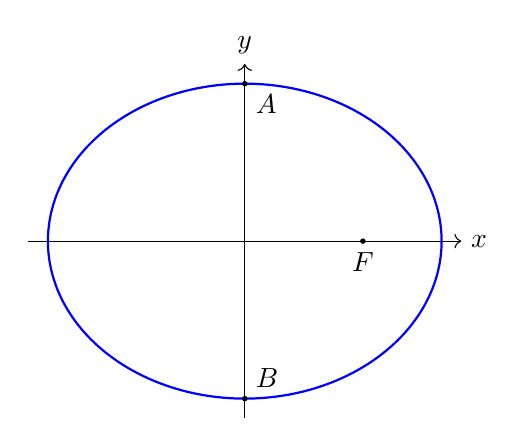
\begin{tikzpicture}[scale=0.5]
      \draw[->] (-5.5,0) -- (5.5,0) node[right] {$x$};
      \draw[->] (0,-4.5) -- (0,4.5) node[above] {$y$};
      \draw[domain=0:2*pi, samples=200,smooth,variable=\t,blue,thick] plot ({5*cos(\t r)},{4*sin(\t r)});
      \node [inner sep=0, outer sep=0, label=270:$F$] (F) at (3,0) {}; 
      \fill [black] (F) circle (2pt); 

      \node [inner sep=0, outer sep=0, label=-45:$A$] (A) at (0,4) {}; 
      \fill [black] (A) circle (2pt); 

      \node [inner sep=0, outer sep=0, label=45:$B$] (B) at (0,-4) {}; 
      \fill [black] (B) circle (2pt); 
    \end{tikzpicture}
  \end{figure}
\emph{Soln:} Since $e = 0.0549$, we have $c = e a$ and $b = \sqrt{a^2-c^2} = \sqrt{1-e^2}a$.

Therefore, the area of $\triangle AFB$ is $2bc/2 = bc = e\sqrt{1-e^2}a^2$.

When the Moon travel counterclockwise from $A$ to $B$, the line connecting the Moon and the Earth will sweep the right half of the ellipse and $\triangle AFB$. Hence, the total area is 
\begin{align*}
  \pi ab /2 + bc = \left(e+\frac{\pi}{2}\right)\sqrt{1-e^2}\times a^2.
\end{align*}
Therefore, from Kepler's second law, the duration is given by
\begin{align*}
  \frac{\pi ab}{27.32} = \frac{\left(e+\frac{\pi}{2}\right)\sqrt{1-e^2}\times a^2}{t}\Rightarrow t = (e/\pi + 0.5)\times 27.32 = 14.14.
\end{align*}
The time from $B$ to $A$ is $27.32 - 14.14 = 13.18$.
\newpage
\item The orbit of Halley comet has an eccentricity of $0.96714$ and its orbital period is 75.32 year. Compute its closest and furthest distance to the sun in terms of Astronomical Unit.

  \emph{Soln:} Suppose the semi-major axis of Halley comet's orbit is $a$. Using Kepler's third law, we have
\begin{align*}
  \frac{75.32^2}{a^3} = \frac{1^2}{1^3}.
\end{align*}
Therefore, $a = 17.835$AU and $c = ea = 17.249$. Hence, the comet is closest to the sun when it is at the vertex close to the sun and the distance is $a-c = 0.586$AU. It is furthest away when it is at the other vertex and the distance is $a+c = 35.084$AU.

\end{enumerate}

\end{document}
%%% Local Variables:
%%% TeX-command-default: "Latexmk"
%%% End:

